\section{Partie 2:Optimisations}

L'ensemble des tests suivants ont étés réalisés sur les calculateurs internes du CERFACS, le Bullx B510 (Neptune) et le LENOVO (nemo). Ils possèdent les caractéristiques suivantes:


\begin{tabular}{|p{3.5cm}|p{5cm}|p{5cm}|}
  \hline
  & Neptune & Nemo \\
  \hline
  Noeuds & 158 & 252 \\
  \hline
  Puissance crête & 53 TFlop/s & 242 TFlop/s \\
  \hline
  Consommation maximale applicative & 51 kW.h & 73 kW.h \\
  \hline
  Consommation à vide & 25 kW.h & 34 kW.h \\
  \hline
  \hline
  Processeurs & Intel Sandy Bridge 8 coeurs (2.6 GHz) & Intel Ivy bridge 12 coeurs (2.5 GHz) \\
  \hline
  Mémoire & 32 Go de mémoire cadencée à 1.6 GHz & 64 Go de mémoire cadencée à 2.1 GHz \\
  \hline

  %%\begin{itemize}
  %%\item 158 noeuds de calculs
  %%\item Puissance crête: 53 TFlop/s
  %%\item Consommation maximale applicative: 51 kW.h
  %%\item Consommation à vide: 25 kW.h
  %%\end{itemize}

  %% Par noeud:
  %% \begin{itemize}
  %% \item 2 processeurs Intel Sandy Bridge 8 coeurs cadencés à 2.6 GHz
  %% \item 32 Go de mémoire cadencée à 1.6 GHz
  %% \end{itemize}
  %% &
  %% \begin{itemize}
  %% \item 252 noeuds de calculs
  %% \item Puissance crête: 242 TFlop/s
  %% \item Consommation maximale applicative: 73 kW.h
  %% \item Consommation à vide: 34 kW.h
  %% \end{itemize}

  %% Par noeud:
  %% \begin{itemize}
  %% \item 2 processeurs Intel Ivy bridge 12 coeurs cadencés à 2.5 GHz
  %% \item 64 Go de mémoire cadencée à 2.1 GHz
  %%\end{itemize} \\
\end{tabular}


\begin{figure}[ht]
  \centering
  \begin{minipage}{.5\textwidth}
    \centering
    \includegraphics[width=.7\linewidth]{figures/neptune.jpg}
    \caption{\label{fig:neptune}Neptune}
  \end{minipage}%
  \begin{minipage}{.5\textwidth}
    \centering
    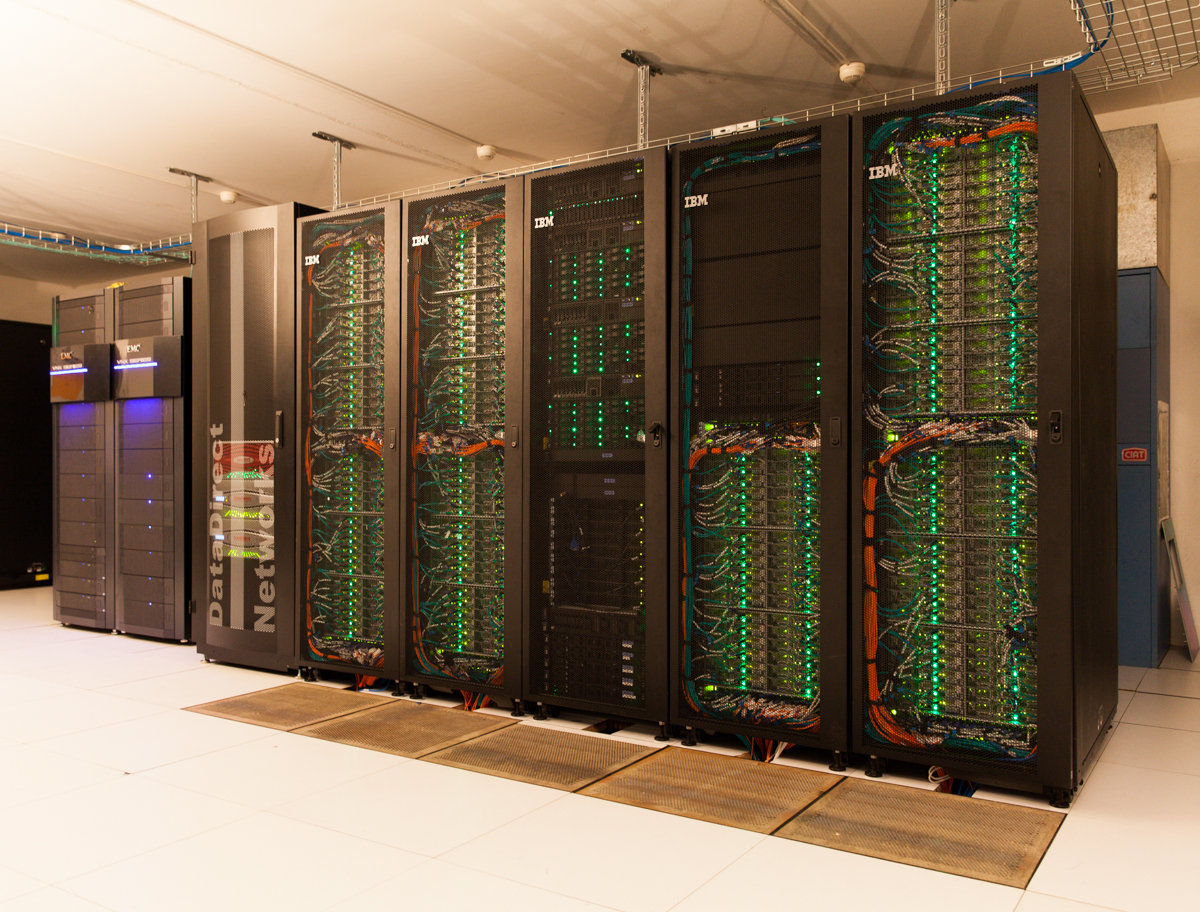
\includegraphics[width=.9\linewidth]{figures/nemo.jpg}
    \caption{\label{fig:neptune_node}Nemo}
  \end{minipage}
\end{figure}



\subsection{Scalaire}
Une fois le programme testé et fonctionnel, j'ai commencé à étudier ses performances. J'ai, dans un premier temps, mesuré un temps de référence pour l'exécution de ce programme; compilation par défaut, donc avec l'option -O2.

\subsubsection{Vectorisation}
J'ai ensuite compiler le programme avec l'option -xAVX qui permet de générer un code vectorisé pour les processeurs possédant l'extension AVX. Pour profiler le programme, j'ai utilisé Intel Advisor qui permet d'analyser la vectorisation d'un programme. Comme on peut le constater sur la figure \ref{fig:advixe}, le compilateur n'a vectorisé qu'un faible pourcentage de boucles (en comparaison avec la référence cf img). Ceci vient du fait que l'ensemble des variables sont contenues dans un unique tableau (fig. \ref{fig:array_s}) et qu'on y accède grâce à des pointeurs. Lorsqu'une boucle doit travailler sur plusieurs tableaux contenus dans ce grand tableau (fig. \ref{fig:o2_avx_novect}), le compilateur assume qu'elle travaille sur un unique grand tableau et empêche donc la vectorisation au profit de la cohérence. Pour résoudre ce problème, il suffit d'indiquer au compilateur qu'il n'y a pas aliasing; on garantit ainsi qu'une zone mémoire ne peut être accédée que par un nom et que le programme ne dépassera pas les limites d'un tableau.


\begin{figure}	
  \centering
  \begin{minipage}{.5\textwidth}
    \centering
    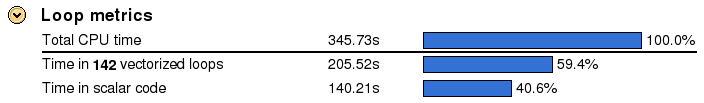
\includegraphics[width=.9\linewidth]{figures/advixe_O2.png}
    \caption{\label{fig:advixe_o2}}
  \end{minipage}%
  \begin{minipage}{.5\textwidth}
    \centering
    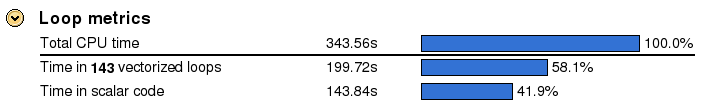
\includegraphics[width=.9\linewidth]{figures/advixe_O2_avx.png}
    \caption{\label{fig:advixe_o2_avx}Caption 2}
  \end{minipage}
  \caption{Répartition des boucles}\label{fig:advixe}
\end{figure}

\begin{figure}[ht]
  \centering
  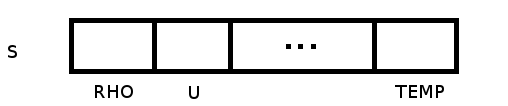
\includegraphics[scale=0.35]{figures/array_s.png}
  \caption{\label{fig:array_s}Structure de la mémoire}
\end{figure}


\begin{figure}[h]
  \centering
  \begin{lstlisting}
    !
    !    DETERMINE THE MASS FRACTION
    !
    DO I=1,NX*NY*NZ
    YK(I)=RHO_Y_TILDE(I,K)/RHO(I)
    END DO
  \end{lstlisting}
  \caption{\label{fig:o2_avx_novect}Boucle non vectorisée}
\end{figure}



\begin{figure}	
  \centering
  \begin{minipage}{.5\textwidth}
    \centering
    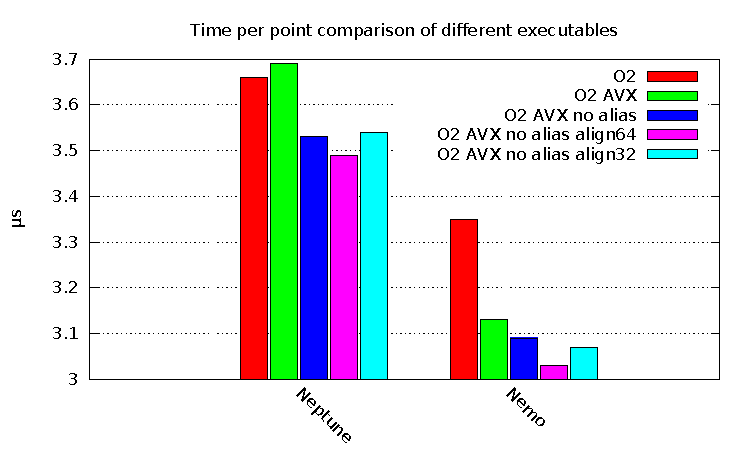
\includegraphics[width=.9\linewidth]{gnuplot/bench_scalaire_per_compute.pdf}
  \end{minipage}%
  \begin{minipage}{.5\textwidth}
    \centering
    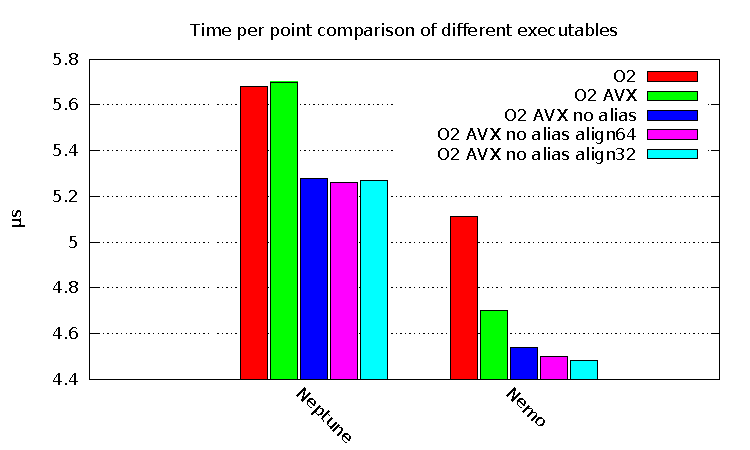
\includegraphics[width=.9\linewidth]{gnuplot/bench_scalaire_per_diag.pdf}
  \end{minipage}
  \caption{Temps par point - Cas périodique}\label{fig:scal_tpp}
\end{figure}


\begin{figure}	
  \centering
  \begin{minipage}{.5\textwidth}
    \centering
    %\includegraphics[width=.9\linewidth]{gnuplot/bench_scalaire_sym_compute.pdf}
    \caption{\label{fig:scal_compute}}
  \end{minipage}%
  \begin{minipage}{.5\textwidth}
    \centering
    %\includegraphics[width=.9\linewidth]{gnuplot/bench_scalaire_sym_diag.pdf}
    \caption{\label{fig:scal_diag}Caption 2}
  \end{minipage}
  \caption{Temps par point - Cas symétrique}\label{fig:scal_tpp}
\end{figure}



\subsubsection{Alignement de la mémoire}
blabla marche pas

\paragraph{durée=f(taille)}

\subsection{MPI}
Comme vu dans l'introduction, l'objectif est de pouvoir faire tourner cette application sur un maillage de taille conséquente ($\approx 10^9$ points). Pour cela, MPI sera utilisé plutôt que OpenMP. En effet, l'approche mémoire partagée oblige à avoir l'ensemble de la mémoire utilisée par l'application au même endroit, hors pour $10^9$ points, la mémoire nécessaire est de l'ordre de 120 Gigaoctets. Les supercalculateurs ne possédant pas autant de mémoire, l'approche MPI paraît plus satisfaisante; chaque processus stockera une partie du domaine ce qui reduira l'utilisation de mémoire.


\paragraph{}Une fois les améliorations scalaires terminée, j'ai commencé à développer une version parallèle de NTMIX. Le but est de diviser le domaine de calcul entre plusieurs processus, chacun calculant ainsi une portion du problème. Cependant, chaque processus ne peut pas travailler de manière totalement indépendante, il est nécessaire d'introduire des points de synchronisations afin que des échanges d'informations se mettent en place:


\begin{itemize}
\item pour le calcul du pas de temps; dans la version séquentielle, un pas de temps maximal est calculé dans le but d'assurer la stabilité de l'algorithme. Dans la version parallèle, chaque processeur devra donc calculer le pas de temps maximal de son sous-domaine et le communiquer aux autres afin de trouver le pas de temps global (opération de réduction).
\item pour le calcul des dérivées; une méthode compacte est utilisée pour calculer les dérivées des différents champs. Une telle méthode implique que la dérivée en un point est dépendante de tous les autres points du domaine. Il sera donc nécessaire d'échanger des informations entre les processus pour ce calcul reste juste.
\end{itemize}


\begin{figure}
\centering
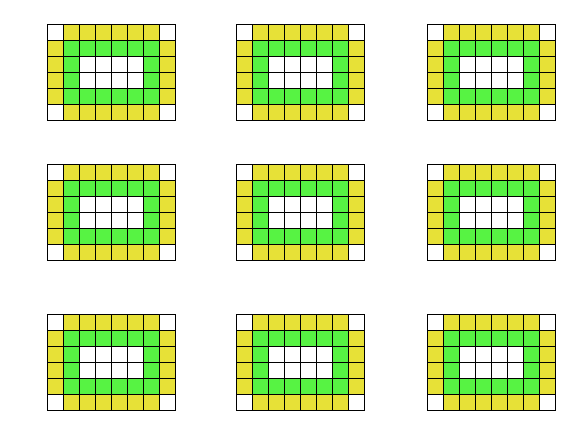
\includegraphics[scale=0.5]{figures/halo.png}
  \caption{\label{fig:neighbor_buf} Motif de communication}
\end{figure}

\subsubsection{Travail réalisé}
Il existe 2 façons de procéder pour le calcul des dérivées:

\begin{itemize}
  \item Recouvrement de domaine
    \begin{itemize}
    \item Un processus reçoit les points des bords de ses voisins
    \item Calcul local des l'évolution des variables
    \item $\nearrow$ Calcul 
    \item 1 grosse communication
    \end{itemize}
  \item Communication pendant le calcul des dérivées
    \begin{itemize}
    \item Un processus calcul uniquement les points de son domaine
    \item Pendant le calcul des dérivées, il reçoit les points de ses voisins
    \item $\searrow$ Calcul 
    \item Plusieurs petites communications
    \end{itemize}
\end{itemize}


\paragraph{Communications}J'ai testé plusieurs de communications pour comparer leurs performance. J'ai dans un premier temps utilisé la fonction MPI\_Neighbor\_alltoallv. Pour l'utiliser, il faut préparer un buffer qui contiendra les données à envoyer à chacun de ses voisins(fig. \ref{fig:neighbor_buf}). La fonction s'occupe elle-même d'envoyer la bonne partie du buffer au bon voisin. Après l'appel à cette fonction, le buffer de réception contient les données de tous les voisins autour d'un processus. Il ne reste plus qu'à stocker les variables reçues à un leur place.

\begin{figure}[ht]
  \centering
  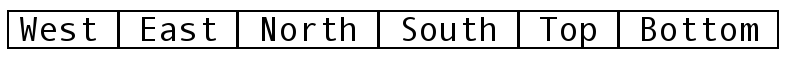
\includegraphics[scale=0.3]{figures/neighbor.png}
  \caption{\label{fig:neighbor_buf} Buffer}
\end{figure}

\paragraph{}X communications points à points/ alternance comm-pack / est-ce que ca recouvre ? 

\subsubsection{Performances}




J'ai donc comparer ces deux méthodes

\paragraph{}temps=f(taille domaine) pour le cas calcul puis plusieurs cas communication (en variant le nombre de procs MPI participant)


\subsubsection{Validation}
Pour s'assurer de l'exactitude des résultats obtenus dans cette version MPI, j'ai fait varié le recouvrement de façon décroissante


\begin{tabular}{|c|c|c||c|c|c|c||c|c|c|}
  \hline
  Overlap & 12 & 11 \\
  \hline
  Mean error & 10E-14 & 10E-10 \\
  \hline
\end{tabular}
